\documentclass[9pt,aspectratio=169]{beamer}

\usepackage{tikz}
\usepackage{datatool}
\usepackage{siunitx-prefix}
% Automatically choosing prefix for SI values (200469 -> 200 k)
\sisetup{round-mode = figures, round-precision = 3}
\DeclareSIUnit{\nothing}{\relax}

\DTLloaddb[noheader]{hours}{hours.csv}
\DTLloaddb[noheader]{jobs}{jobs.csv}

\setbeamercolor{normal text}{fg=white}
\usebeamercolor[fg]{normal text}
\setbeamercolor{item}{fg=white}
\setbeamercolor{structure}{fg=white}
\setbeamercolor{block title}{bg=black,fg=white}
\setbeamercolor{block body}{bg=black,fg=white}
\setbeamercolor{box1}{bg=black,fg=white}
\usebackgroundtemplate%
{%
    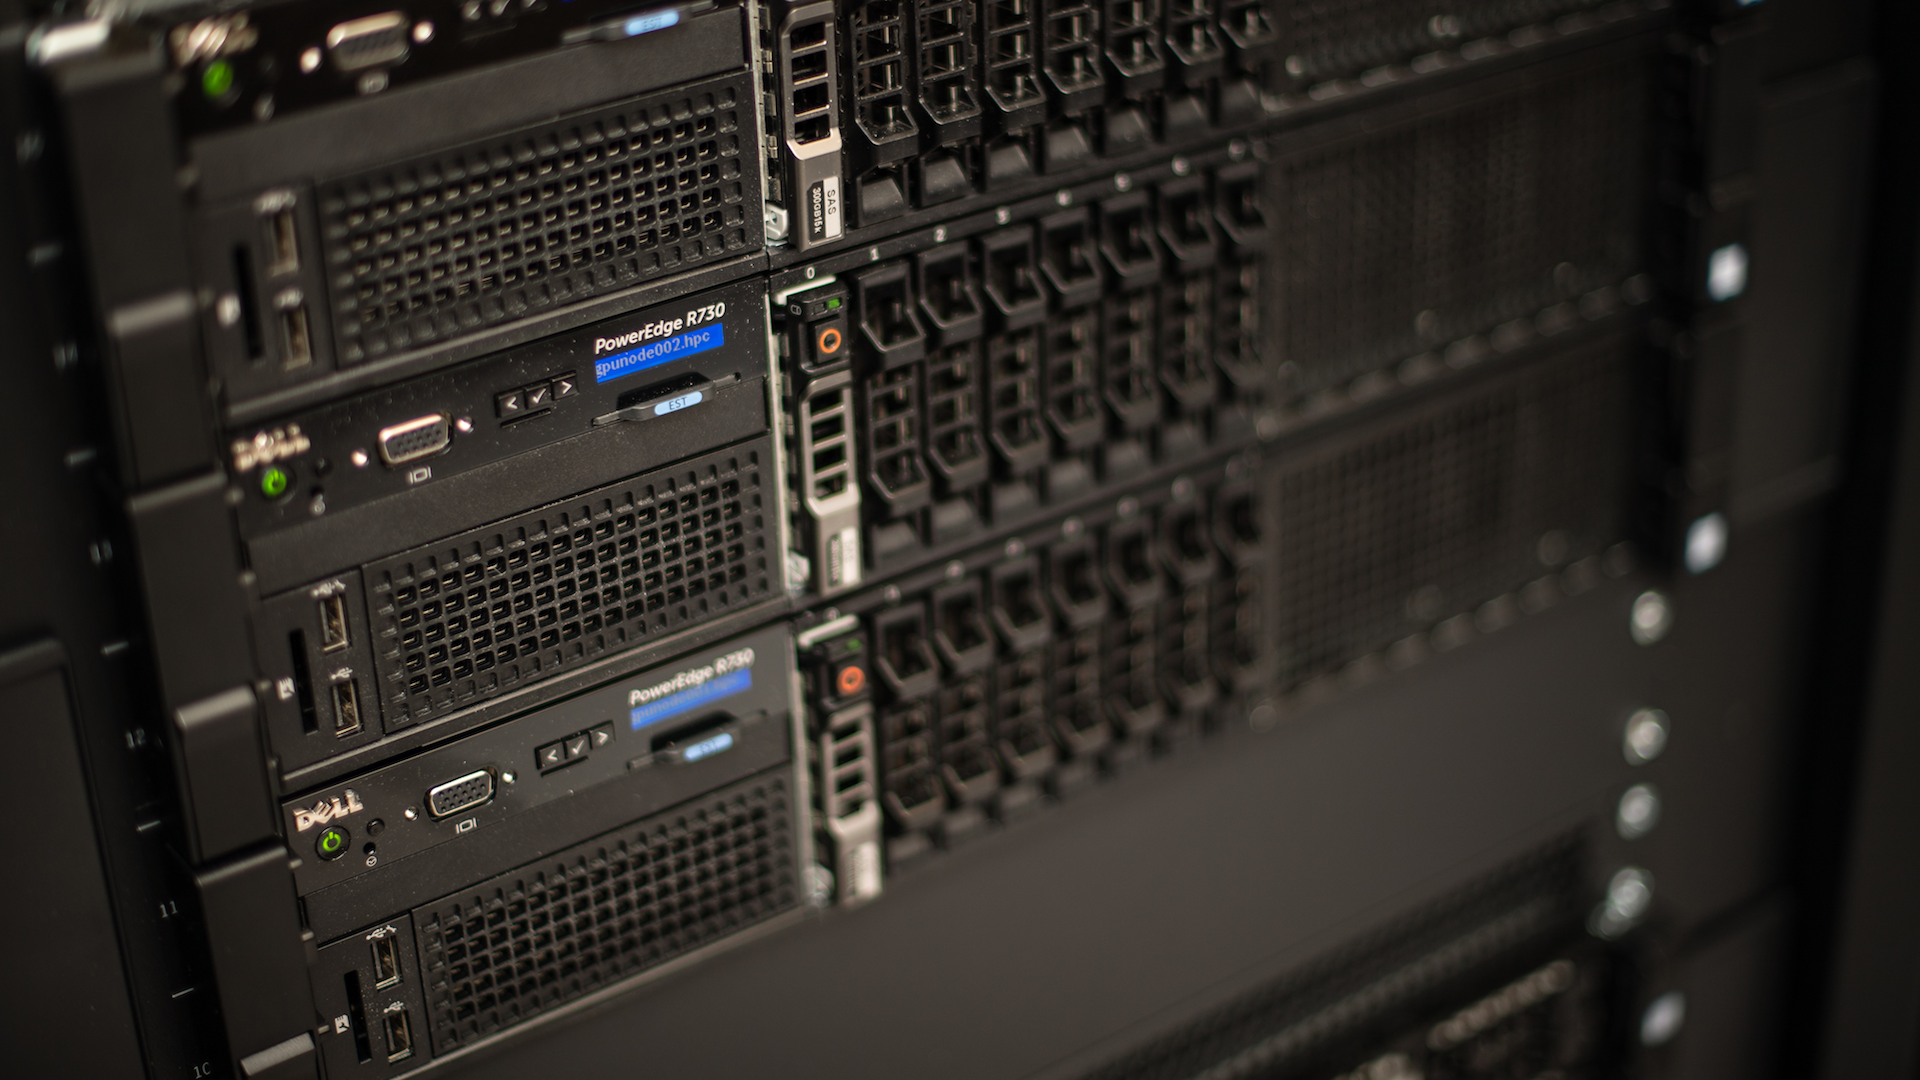
\includegraphics[width=\paperwidth,height=\paperheight]{hpc-background}%
}
\newlength{\navigationsymbolheight}
\newcommand{\highopacity}{1.0}
\newcommand{\lowopacity}{0.65}
\newenvironment{opaque}{\pgfsetfillopacity{\highopacity}}{\pgfsetfillopacity{\lowopacity}}
\settoheight{\navigationsymbolheight}{\NoHyper\insertframenavigationsymbol}
% In case we need to adjust an image or logo placement to use space left by removing navigation symbols
\setbeamertemplate{navigation symbols}{}
\begin{document}
\begin{frame}
  \pgfsetfillopacity{\lowopacity}
  \begin{columns}[t]
    \begin{column}{0.49\textwidth}
      
      \begin{block}{\begin{opaque}\textbf{Very} Brief Introduction to High Performance Computing at Tennessee Tech\end{opaque}}
      \end{block}
      \begin{block}{\begin{opaque}Mike Renfro, PhD: \href{mailto:renfro@tntech.edu}{renfro@tntech.edu}\end{opaque}}
        \begin{opaque}\begin{itemize}
          \item \href{https://www.hpc.tntech.edu/}{www.hpc.tntech.edu}
          \item HPC Systems Administrator
          \item NSF XSEDE Campus Champion
        \end{itemize}\end{opaque}
      \end{block}
      \begin{block}{\begin{opaque}Hardware:\end{opaque}}
      \begin{opaque}\begin{itemize}
        \item 44 28-core compute servers, including 8 GPUs
        \item 64--896 GB RAM per server
      \end{itemize}\end{opaque}
      \end{block}
      \begin{block}{\begin{opaque}OS and Software:\end{opaque}}
        \begin{opaque}\begin{itemize}
          \item Red Hat and CentOS Linux
          \item Lots of installed applications (and you can add some of your own)
        \end{itemize}\end{opaque}
      \end{block}
  \end{column}
    \begin{column}{0.49\textwidth}
      \begin{block}{\begin{opaque}Usage to date:\end{opaque}}
        \centering
        \begin{tikzpicture}
          \begin{opaque}
          \node[anchor=south west,inner sep=0] (image) at (0,0) {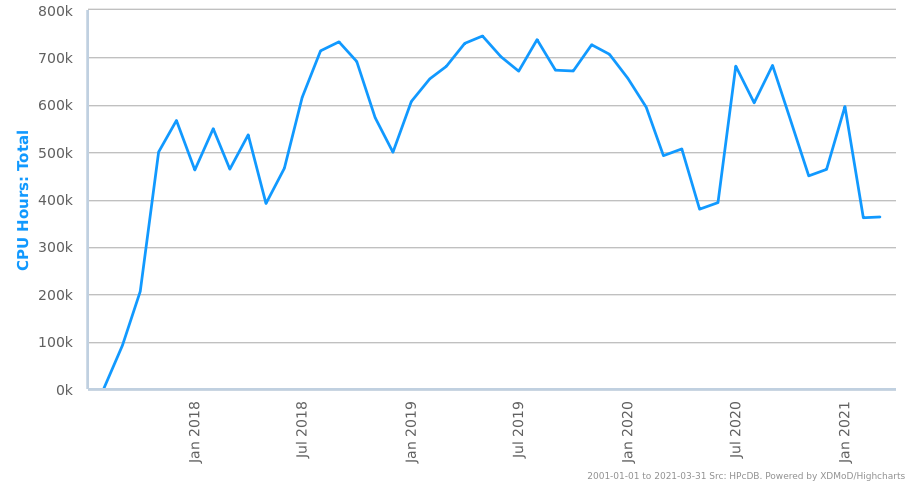
\includegraphics[width=0.35\paperwidth]{hpc-usage}};
          \end{opaque}
          \begin{scope}[x={(image.south east)},y={(image.north west)}]
            \node[align=center,black] at (0.6, 0.45) {{\DTLforeach{jobs}{\totaljobs=Column1}{\prefixSI{\totaljobs}{\prefix\nothing}}}
 jobs completed,\\ \DTLforeach{hours}{\totalcpuhours=Column1}{\prefixSI{\totalcpuhours}{\prefix\nothing}}
 CPU-hours delivered};
          \end{scope}
        \end{tikzpicture}
      \end{block}
      \begin{block}{\begin{opaque}Common job types:\end{opaque}}
        \begin{opaque}\begin{itemize}
          \item Molecular dynamics
          \item Computational fluid dynamics
          \item Artificial intelligence/machine learning
          \item Nuclear physics
          \item Genomics
          \item Environmental science
          \item Computational solid mechanics
        \end{itemize}\end{opaque}
      \end{block}
    \end{column}
  \end{columns}
\end{frame}
\end{document}
